\begin{tcolorbox}[title={\Large グラフの教師あり分類問題}]
	\structure{入力}
	クラス($ y = \plus \mbox{~or~} \minus $)の分かる複数のグラフ $N$ 個
	\vspace{20px}

	\begin{textblock*}{0.2\textwidth}(50pt,0pt)
		\begin{center}
			$\plus$ \\
			\includegraphics[width=0.6\textwidth]{img/graph/g01r.png}
		\end{center}
	\end{textblock*}

	\begin{textblock*}{0.2\textwidth}(250pt,0pt)
		\begin{center}
			$\plus$ \\
			\includegraphics[width=0.6\textwidth]{img/graph/g02r.png}
		\end{center}
	\end{textblock*}

	\begin{textblock*}{0.2\textwidth}(450pt,0pt)
		\begin{center}
			$\plus$ \\
			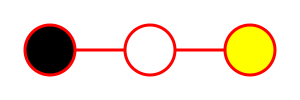
\includegraphics[width=0.6\textwidth]{img/graph/g03r.png}
		\end{center}
	\end{textblock*}

	\begin{textblock*}{0.2\textwidth}(650pt,0pt)
		\begin{center}
			$\minus$ \\
			\includegraphics[width=0.6\textwidth]{img/graph/g04b.png}
		\end{center}
	\end{textblock*}

	\begin{textblock*}{0.2\textwidth}(50pt,150pt)
		\begin{center}
			$\minus$ \\
			\includegraphics[width=0.6\textwidth]{img/graph/g05b.png}
		\end{center}
	\end{textblock*}

	\begin{textblock*}{0.2\textwidth}(250pt,150pt)
		\begin{center}
			$\minus$ \\
			\includegraphics[width=0.6\textwidth]{img/graph/g06b.png}
		\end{center}
	\end{textblock*}

	\begin{textblock*}{0.2\textwidth}(450pt,150pt)
		\begin{center}
			$\plus$ \\
			\includegraphics[width=0.6\textwidth]{img/graph/g07r.png}
		\end{center}
	\end{textblock*}

	\begin{textblock*}{0.2\textwidth}(650pt,150pt)
		\begin{center}
			$\minus$ \\
			\includegraphics[width=0.6\textwidth]{img/graph/g08b.png}
		\end{center}
	\end{textblock*}

	\vspace{350px}

	\structure{出力}
	クラスを予測する分類森 $F$ \\
	\begin{textblock*}{0.45\textwidth}(0.6\hsize,-80pt)
		\includegraphics[width=0.8\textwidth]{img/dt.png}
	\end{textblock*}
	\begin{minipage}[t]{0.45\hsize}
		\begin{center}
			\includegraphics[width=0.24\textwidth]{img/graph/g09.png}
			\raisebox{30px}{$ \Rightarrow F \Rightarrow \plus \mbox{~or~} \minus $} \\
			\[
				F_t(x) = \sum_{i=1}^{t} f_i(x) = \sum_{i=1}^{t} \sum_{v \in \mbox{\footnotesize leaves of }f_i} w_v r_v
			\]
		\end{center}
	\end{minipage} \\
	\vspace{50pt}

	\structure{特徴ベクトル} 部分グラフの有無
	\begin{table}
		\begin{tabular}[b]{l|ccccr}
			&	
			\includegraphics[width=0.1\textwidth]{img/subgraph/kw.png} &
			\includegraphics[width=0.1\textwidth]{img/subgraph/kwg.png} &
			\raisebox{10px}{\includegraphics[width=0.1\textwidth]{img/subgraph/kwgy.png}} &
			\includegraphics[width=0.1\textwidth]{img/subgraph/wg.png} &
			\raisebox{30px}{$\dots$} \\
			\hline
			\hline
			\raisebox{-.3\height}{\includegraphics[width=0.12\textwidth]{img/graph/g01r.png}}	& 0 & 0 & 0 & 1 & \\
			\raisebox{-.3\height}{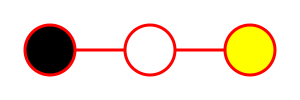
\includegraphics[width=0.12\textwidth]{img/graph/g03r.png}}	& 1 & 0 & 0 & 0 & \\
			\raisebox{-.5\height}{\includegraphics[width=0.12\textwidth]{img/graph/g05b.png}}	& 1 & 1 & 0 & 1 & \\
			\raisebox{-.5\height}{\includegraphics[width=0.12\textwidth]{img/graph/g07r.png}}	& 1 & 1 & 1 & 1 & \\
		\end{tabular}
	\end{table}
	\begin{tcolorbox}[colframe=white,colback=white,left=30px]
		全ての部分グラフに関して有無を調べるのは困難 \\
		頻出する部分グラフのみ調べる方法もあるが、 \\
		\alert{可能なら全ての部分グラフを活用したい!} \\
		GBDT なら可能だが精度が悪い。XGBoost, RGF でもしたい。
	\end{tcolorbox}
\end{tcolorbox}
